\chapter{Theoretical Background}
\label{Theoretical Background}

\section*{Generative Adversarial Nets}

Generative Adversarial Networks (GANs) consist of a generator G and a discriminator D, 
both implemented using artificial neural networks. The parametrization of GANs involves 
defining the network structure of these components and initializing their weights and biases \citep{10.1007/s10928-021-09787-4}. 
The success of GANs relies on balancing the training of these two networks, where the 
G aims to produce samples $G(z)$ that mimic real data distributions $p_{data}(x)$ by input noise z, while the D 
learns to differentiate between real and generated samples \citep{10.1109/taslp.2017.2761547}. 
The training process involves iteratively updating the weights and biases of the networks through 
adversarial training, where the generator tries to deceive the discriminator, and the discriminator 
aims to accurately classify samples \citep{10.48550/arxiv.1802.05637}.

\begin{equation}
    \min_{G} \max_{D} V(D, G) = \mathbb{E}_{x \sim p_{data}(x)} [\log D(x)] + \mathbb{E}_{z \sim p_{z}(z)} [\log(1 - D(G(z)))].
\end{equation}


The formula 3.1 is the objective function of Generative Adversarial Networks (GANs). 
It describes the game process between the Generator (G) and the Discriminator (D). Specifically, the formula defines a minimax game between the Discriminator and the Generator.

\begin{itemize}
    \item \textbf{ $D(G(z))$:} is the output of the discriminator for the data G(z) generated by the generator. Indicating the probability that the discriminator believes that the generated data comes from the real data distribution.
    \item \textbf{$D(x)$:} is the output of the discriminator for the real data x. Indicating the probability that the discriminator believes that the real data x comes from the real data distribution.
    \item \textbf{ $x \sim p_{data}(x)$:} means that sample x is drawn from the true data distribution $p_{data}$.
    \item \textbf{ $z \sim p_{z}(z)$:} means that sample z is drawn from the fake data distribution $p_{z}$.
    \item \textbf{$\mathbb{E}{_x \sim p_{data}(x)}[\log D(x)]$:} means taking the average value of $\log D(x)$ for all samples x on the true data distribution $p_{data}(x)$.
    \item \textbf{$\mathbb{E}{x \sim p_{z}(z)}[\log (1 - D(x))]$:} means taking the average value of $\log (1 - D(G(z)))$ for all samples z on the noise distribution $p_z(z)$.
\end{itemize}




D(G(z)) is the output of the discriminator for the data G(z) generated by the generator, 
indicating the probability that the discriminator believes that the generated data comes from the real data distribution.
D(x) is the output of the discriminator for the real data x, 
indicating the probability that the discriminator believes that the real data x comes from the real data distribution.

$\mathbb{E}{x \sim p_{data}(x)}[\log D(x)]$ represents the average value of $\log D(x)$ for all samples x on the true data distribution $p_{data}(x)$.
$x \sim p_{data}(x)$ means that sample x is drawn from the true data distribution $p_{data}$.
$\log D(x)$ is the logarithm of the output of the discriminator D for the input x.


\begin{equation}
    \max_{D} V(D, G) = \mathbb{E}_{x \sim p_{data}(x)} [\log D(x)] + \mathbb{E}_{z \sim p_{z}(z)} [\log(1 - D(G(z)))].
\end{equation}

The formula 3.2 shows, the discriminator tries to maximize V(D, G).

\begin{equation}
    \min_{G} V(D, G) = \mathbb{E}_{z \sim p_{z}(z)} [\log(1 - D(G(z)))].
\end{equation}


The formula 3.3 shows, the generator tries to minimize V(D, G). 
This means that the generator tries to generate realistic data G(z) so that the discriminator cannot distinguish 
them from real data, that is: It is hoped that D(G(z)) is close to 1, so that $\log (1 - D(G(z)))$ is closer to negative infinity.
This dynamic equilibrium drives the GAN framework towards generating outputs that closely resemble authentic data, 
fulfilling the objective of producing realistic data that is challenging to distinguish from real data.


\begin{equation}
    \min_{G} V(D, G) = \mathbb{E}_{z \sim p_{z}(z)} [-\log(D(G(z)))].
\end{equation}

In real training process, the formula 3.3 will replace by 3.4. Since, when the discriminator D is strong, 
the gradient of the $log(1 - D(G(z)))$ approaches zero, leading to slow generator training and diminished gradient update impact \citep{10.1007/s11263-019-01265-2}.  
This approach ensures that the gradient of the logarithm is large, providing the generator with more effective gradient updates and 
helping to avoid the vanishing gradient issue \citep{10.1109/tpami.2018.2872043}.



The GAN network parameters play a crucial role in determining the quality and diversity of 
the generated samples $G(x)$ \citep{10.1007/s10928-021-09787-4}. The optimization process in GANs 
typically involves minimizing a min-max function to ensure the G produces samples that 
are indistinguishable from real data \citep{10.1109/taslp.2017.2761547}. Maintaining this balance 
during training is essential for achieving high-quality sample generation \citep{10.1007/s10928-021-09787-4}. 
The D's role is to provide feedback to the generator by acting as a critic, 
guiding the G towards producing more realistic samples \citep{10.48550/arxiv.1802.05637}.



\section*{Optimal Discriminator}

The training process of Generative Adversarial Networks (GANs) is inherently adversarial. 
The generator endeavors to create increasingly realistic fake samples to deceive the discriminator, 
while the discriminator seeks to more accurately distinguish between real and fake samples. 
To understand how this process works, in the following sections, 
I will describe the GAN training process from the perspectives of data distribution and mathematical formulation.

\subsection*{Distribution Angle}



\begin{figure}[H]
    \centering
    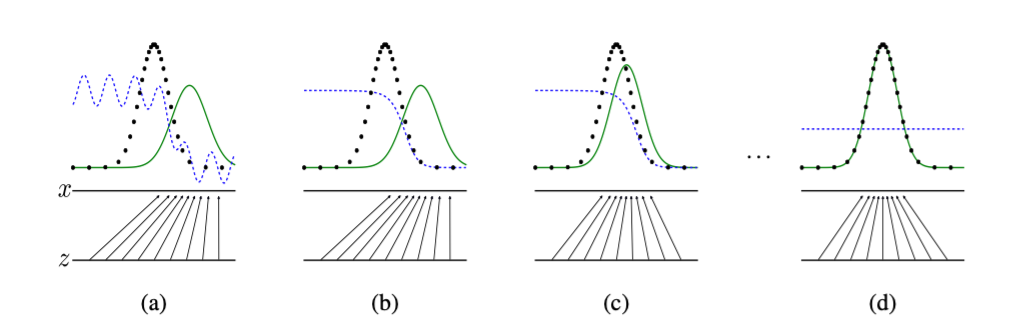
\includegraphics[width=1.2\linewidth]{./Images/data_distribution.jpg}
    \caption{Diagram of GAN training process}
    \label{fig:my_picture}
    \vspace{1pt} % Vertical space, optional
    \small{Source: \cite{goodfellow2014generative}}
\end{figure}


\begin{itemize}
    \item \textbf{ Green Curve:} Represents the distribution of generated samples. Initially, the distribution of generated samples may differ significantly from the real samples. As training progresses, the generated samples’ distribution gradually approaches that of the real samples.
    \item \textbf{Black Dots:} Represent the distribution of real samples. These points remain unchanged throughout the training process and represent the target distribution.
    \item \textbf{ Blue Line:} Represents error or noise. Initially, the error is large and manifests as a wavy sine curve. As training progresses, the error gradually decreases, and the blue line becomes increasingly flat.
    \item \textbf{ Lines Arranged Below (Labeled as x and z):} Represent the distribution of samples in the latent space. In GAN training, samples from the latent space are mapped to the data space through the generator, producing corresponding samples.
\end{itemize}


During the training process of the GAN model, the generator and the discriminator fight against each other. 
The generator tries to produce realistic samples to fool the discriminator, while the discriminator strives 
to distinguish real samples from generated samples. Initially, the generator generates samples with poor 
quality and large errors, similar to the blue sine wave in Figure (a). However, as training proceeds and 
the generator continues to improve, the error in generated samples gradually decreases, similar to the 
blue lines in figures (b) and (c) becoming flat. At the same time, the distribution of real samples and 
generated samples gradually becomes consistent, and finally reaches the optimal state in Figure (d). At this moment $p_{data}(x) = p_g(x)$, 
the samples generated by the generator are almost the same as the real samples, and the error is minimized. 
During the entire process, the sample distribution gradually converges from the initial noise and discrete 
state to a state that highly coincides with the real distribution, reflecting a significant improvement in 
the quality of the generated samples.


\subsection*{Formula Angle}


1. Problem Setup

In a Generative Adversarial Network (GAN), the objective is to train a generator \( G \) and a discriminator \( D \) to generate data that resembles the real data distribution. The objective function to be maximized is given by:

\begin{equation}
    V(D, G) = \mathbb{E}_{\mathbf{x} \sim p_{\text{data}}(\mathbf{x})} [\log D(\mathbf{x})] + \mathbb{E}_{\mathbf{z} \sim p_{\mathbf{z}}(\mathbf{z})} [\log (1 - D(G(\mathbf{z})))].
\end{equation}

2. Rewriting the Objective Function

First, the objective function is rewritten in integral form:

\begin{equation}
    V(D, G) = \int p_{\text{data}}(\mathbf{x}) \log D(\mathbf{x}) \, d\mathbf{x} + \int p_{\mathbf{z}}(\mathbf{z}) \log (1 - D(G(\mathbf{z}))) \, d\mathbf{z}.
\end{equation}

By changing variables \(\mathbf{x}' = G(\mathbf{z})\), the second term can be rewritten as an integral over the generated data distribution \( p_g(\mathbf{x}) \):

\begin{equation}
    \int p_g(\mathbf{x}) \log (1 - D(\mathbf{x})) \, d\mathbf{x}.
\end{equation}

Thus, the objective function becomes:

\begin{equation}
    V(D, G) = \int \left[ p_{\text{data}}(\mathbf{x}) \log D(\mathbf{x}) + p_g(\mathbf{x}) \log (1 - D(\mathbf{x})) \right] d\mathbf{x}.
\end{equation}

3. Deriving the Optimal Discriminator

To find the optimal discriminator \( D^* \), it needs to take the derivative of the objective function with respect to \( D(\mathbf{x}) \) and set it to zero.

Let:

\begin{equation}
    f(D(\mathbf{x})) = p_{\text{data}}(\mathbf{x}) \log D(\mathbf{x}) + p_g(\mathbf{x}) \log (1 - D(\mathbf{x})).
\end{equation}

Taking the derivative with respect to \( D(\mathbf{x}) \):

\begin{equation}
    \frac{d}{dD(\mathbf{x})} f(D(\mathbf{x})) = \frac{p_{\text{data}}(\mathbf{x})}{D(\mathbf{x})} - \frac{p_g(\mathbf{x})}{1 - D(\mathbf{x})}.
\end{equation}

Setting the derivative to zero:

\begin{equation}
    \frac{p_{\text{data}}(\mathbf{x})}{D(\mathbf{x})} = \frac{p_g(\mathbf{x})}{1 - D(\mathbf{x})}.
\end{equation}

Solving this equation:

\begin{equation}
    p_{\text{data}}(\mathbf{x})(1 - D(\mathbf{x})) = p_g(\mathbf{x})D(\mathbf{x}),
\end{equation}

\begin{equation}
    p_{\text{data}}(\mathbf{x}) - p_{\text{data}}(\mathbf{x})D(\mathbf{x}) = p_g(\mathbf{x})D(\mathbf{x}),
\end{equation}

\begin{equation}
    p_{\text{data}}(\mathbf{x}) = p_{\text{data}}(\mathbf{x})D(\mathbf{x}) + p_g(\mathbf{x})D(\mathbf{x}),
\end{equation}

\begin{equation}
    p_{\text{data}}(\mathbf{x}) = D(\mathbf{x})(p_{\text{data}}(\mathbf{x}) + p_g(\mathbf{x})),
\end{equation}

\begin{equation}
    D(\mathbf{x}) = \frac{p_{\text{data}}(\mathbf{x})}{p_{\text{data}}(\mathbf{x}) + p_g(\mathbf{x})}.
\end{equation}

4. Optimal Discriminator Formula

Therefore, the optimal discriminator \( D^* \) is given by:

\begin{equation}
    D^*(\mathbf{x}) = \frac{p_{\text{data}}(\mathbf{x})}{p_{\text{data}}(\mathbf{x}) + p_g(\mathbf{x})}.
\end{equation}


\begin{itemize}
    \item When $p_{\text{data}}(x)$ is much larger than $p_g(x), D^*_G(x) \approx 1$, indicating that the data point is almost certainly from the real data.
    \item When $p_{\text{data}}(x)$ is much smaller than $p_g(x), D^*_G(x) \approx 0$, indicating that the data point is almost certainly from the generated data.
    \item When $p_{\text{data}}(x)$ is close to $p_g(x), D^*_G(x) \approx 0.5$, indicating that the data point has a 50% chance of coming from the real data and a 50% chance of coming from the generated data.
\end{itemize}


5. Verifying the Optimal Discriminator

To verify that this \( D^* \) maximizes the objective function, substitute \( D^* \) back into the objective function:

\begin{equation}
    V(D^*, G) = \int \left[ p_{\text{data}}(\mathbf{x}) \log \left( \frac{p_{\text{data}}(\mathbf{x})}{p_{\text{data}}(\mathbf{x}) + p_g(\mathbf{x})} \right) + p_g(\mathbf{x}) \log \left( 1 - \frac{p_{\text{data}}(\mathbf{x})}{p_{\text{data}}(\mathbf{x}) + p_g(\mathbf{x})} \right) \right] d\mathbf{x}.
\end{equation}

Since:

\begin{equation}
    1 - D^*(\mathbf{x}) = 1 - \frac{p_{\text{data}}(\mathbf{x})}{p_{\text{data}}(\mathbf{x}) + p_g(\mathbf{x})} = \frac{p_g(\mathbf{x})}{p_{\text{data}}(\mathbf{x}) + p_g(\mathbf{x})},
\end{equation}

substituting this in:

\begin{equation}
    V(D^*, G) = \int \left[ p_{\text{data}}(\mathbf{x}) \log \left( \frac{p_{\text{data}}(\mathbf{x})}{p_{\text{data}}(\mathbf{x}) + p_g(\mathbf{x})} \right) + p_g(\mathbf{x}) \log \left( \frac{p_g(\mathbf{x})}{p_{\text{data}}(\mathbf{x}) + p_g(\mathbf{x})} \right) \right] d\mathbf{x}.
\end{equation}

This objective function represents the negative of the cross-entropy, which is maximized when \( D(\mathbf{x}) = D^*(\mathbf{x}) \). The cross-entropy is minimized by maximizing the similarity between the true distribution and the predicted distribution, so its negative is maximized at the same point.

6. Conclusion

Through the above derivation, it has shown that given the generator \( G \), the optimal form of the discriminator \( D \) is:

\begin{equation}
    D^*(\mathbf{x}) = \frac{p_{\text{data}}(\mathbf{x})}{p_{\text{data}}(\mathbf{x}) + p_g(\mathbf{x})}.
\end{equation}

This demonstrates that the optimal discriminator \( D^* \) outputs the probability that the input data comes from the real data distribution. This formula provides a theoretical foundation for training GANs, guiding the updates to the generator \( G \) so that its generated data gradually approaches the real data distribution.


\subsection*{Measuring performance of GAN}


Fréchet Inception Distance (FID) is a metric commonly used in Generative Adversarial Network (GAN) models 
to quantify the dissimilarity between two image distributions \citep{10.48550/arxiv.2203.06026}. 
It measures the distance between the distributions of real images and generated images, providing 
a numerical assessment of the quality of generated images. FID has gained prominence in evaluating 
the performance of GANs due to its ability to capture both the quality and diversity of generated images \citep{10.3390/app12157599}.

A lower FID value indicates that the distribution of the generated images is closer to that of real images, 
reflecting higher quality and diversity in the generated images \citep{10.1117/12.2673366}. 
Specifically, a FID value below 10 is considered to represent very high-quality generated images, 
while values between 10 and 50 indicate good quality, and values above 50 suggest average or poor quality \citep{10.1117/12.2673366}.


\begin{equation}
    \text{FID} = || \mu_r - \mu_g ||^2 + \text{Tr}(\Sigma_r + \Sigma_g - 2(\Sigma_r \Sigma_g)^{1/2})
\end{equation}


\begin{equation}
    \mu_r = \frac{1}{N} \sum_{i=1}^{N} f(x_i), \quad \Sigma_r = \frac{1}{N} \sum_{i=1}^{N} (f(x_i) - \mu_r)(f(x_i) - \mu_r)^T
\end{equation}

\begin{equation}
    \mu_g = \frac{1}{M} \sum_{i=1}^{M} f(G(z_i)), \quad \Sigma_g = \frac{1}{M} \sum_{i=1}^{M} (f(G(z_i)) - \mu_g)(f(G(z_i)) - \mu_g)^T
\end{equation}


\begin{itemize}
    \item \textbf{ $\mu_r \text{ and } \mu_g$:}  are the feature means of the real and generated images, respectively.
    \item \textbf{$\Sigma_r \text{ and } \Sigma_g$:}  are the feature covariance matrices of the real and generated images, respectively.
    \item \textbf{ $\text{Tr}$:}  represents the trace (the sum of the diagonal elements of the matrix).
\end{itemize}


\subsection*{Why Not Accuracy}

Accuracy is not suitable for evaluating GANs because accuracy is an indicator of classification tasks, 
which is used to measure the prediction accuracy of the model in classification tasks, and cannot 
measure the quality and diversity of generated data. In generation tasks, there is no clear 
"correct answer" and the generated data has no "real label", so it is impossible to directly 
compare the correspondence between the generated data and a real sample. 

FID (Fréchet Inception Distance) quantifies the difference between generated data and real 
data by comparing their distribution in the Inception network feature space. FID takes into 
account the overall distribution of generated data and real data, and can reflect the quality 
and diversity of generated data. A low FID value indicates that the distribution of generated 
data is very close to the distribution of real data, that is, the generated data is both realistic 
and diverse, so FID is a more suitable indicator for evaluating the performance of generative models.